\section{Overview}
The Project Scope, detailed in the previous chapter, requires that the DoodleBot Team design and implement a system that can take an input in the form of a bitmap image and reproduce this image on paper using the provided hardware. 

In addition to the requirements, the DoodleBot team designed the system to another key performance indicator - minimizing for the machine to draw.



\begin{figure}  
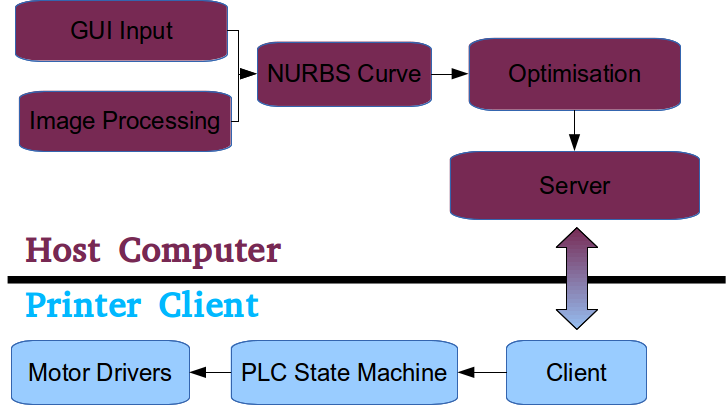
\includegraphics[width=\textwidth]{figures/introduction/system.png}
\caption[System Architecture]{
\label{fig:system}}
\end{figure}

\subsubsection{User Interface} 
The main Graphical User Interface (GUI) is written in the Java programming language. This language was chosen for the simplicity and level of library support that it gives graphical interfaces, as well as the power that the language has to easily create servers and to interface with other programming languages. The desired result for this module was to allow for user input and manipulation of curve objects that would then be drawn by the printer at the users request. This was achieved through use of the Swing package, which comes with features that are ready made to allow for the drawing of different types of curves. The user directly manipulates the control points of a curve, with the shape of the curve updating in real time. 

\subsubsection{Image Processing}
The image input method consists of a MATLAB\textsuperscript{\textregistered} script that the Java GUI can call, which processes a given image and returns a series of URBS curves. These can then be displayed with the main GUI. The MATLAB\textsuperscript{\textregistered} script performs this task by applying some initial image equalisation and filtering before running a Canny edge detector. The resulting output has all of the detected edges collated into 'edge objects' - line segments that do not split into two separate lines. These edge objects are then simplified by approximation by straight lines, before being fitted to a NURBS curve in a way that tries to minimise error.

\subsubsection{URBS Curve}
The key data structure that most modules on the Host utilise is a 3rd order Uniform Rational Basis Spline (URBS) curve. An URBS curve is a cousin of the better known NURBS curve, with the only difference being that the knot vector of the URBS curve has its knots uniformly spaced. An URBS curve is a method of representing an arbitrary curve through a space with a minimal set of data values. Curves can subsequently have any number of points on their surface calculated to arbitrary precision. There are a few major benefits to the restriction of input lines to 3rd order URBS curves which result in nice properties for our subsequent optimisation task; namely continuous velocity across the domain of the curve and uniform division of the path space resulting in an even division of optimisation between each pair of control points.

\subsubsection{Optimisation}
This module was solved with the application of a MATLAB script that programs the given URBS curve into a discrete structure that can be solved by SeDuMi. The script performs a change of variables in order to linearise the physical constraints of the system. The change of variables retains the convexity of the optimisation cost for which we wish to solve. The script also restricts the otherwise infinite dimensionality of the function we wish to solve for to a piecewise approximation. This means the result of our solution will be an approximation of the true and infinite dimensional optimum for our given cost. 
The problem we wish to solve is; given a path 
\begin{align*}
\textbf{q}(s) = 
\begin{bmatrix}
  x(s)\\
  y(s)
 \end{bmatrix}
\end{align*}
We would like to determine the maximal $\frac{ds(t)}{dt}$ for each point in time, subject to the actuator limitations of our plant. This maximal $\frac{ds(t)}{dt}$ will result in the traversal of the path $\textbf{q}(s)$ in the minimum possible time. The key restriction that our model faces is the selection of the path velocity $\frac{ds(t)}{dt} = \dot{s}(t)$ that will allow the curve's trajectory to be within the actuator limitations for both axes. The torque required by each actuator at a given point on a given curve is dependent on the shape of the curve and the path velocity $\dot{s}(t)$. Due to the Bang-Bang nature of the time optimal problem we wish to solve, one actuator will be limiting the maximum $\dot{s}(t)$ at each point along the curve. The optimisation algorithm will determine the limiting actuator and generate a piecewise path velocity that obeys that actuator constraint.

\subsubsection{Server}
The implementation of the transmission of the optimal path from Server to Client was given to be a transmission of the velocity instructions that the PLC should give to its motors at a given uniform distribution of sample times. The PLC could linearly accelerate the motors to those velocities to achieve a good approximation of the curve to be followed. This was implemented as a result of limitations on the frequency of velocity instructions given by the PLC and also to simplify the code required to be written on the PLC side. This technique was simulated to result in a high accuracy for a sufficiently high instruction frequency.

\subsubsection{Client}
\subsubsection{PLC State Machine}
\subsubsection{Motor Drivers}



